The implementation supports three distinct initial conditions for the scalar field and its canonical momentum. These include a plane wave, an exact Gaussian, and a multipolar Gaussian function. The plane wave and exact Gaussian initial data were developed for the purpose of testing multipatch derivatives in flat spacetime, which will be elaborated on further in subsequent sections. The exact Gaussian initial data is named as such to reflect the fact that it is an exact solution of the Klein-Gordon equation in flat spacetime.

The multipolar Gaussian function is a basic Gaussian function that is multiplied by a linear combination of real spherical harmonics. This particular function was the one chosen during our ``production'' runs as it has the ability to excite specific modes in the system based on the chosen parameters for the linear combination. The development of this initial data is based on the methodology presented in Ref.~\cite{PhysRevD.87.043513}. In order to construct it, let us first introduce its components. We start with the Gaussian function $G(r, \sigma)$, given by
%
\begin{equation}
  G(r, \sigma) = \exp\left( -\frac{1}{2} \left( \frac{r}{\sigma} \right)^2  \right).
  \label{eq:wave_scattering_gaussian}
\end{equation}
%
where $\sigma$ is the Gaussian width parameter. Next, we introduce the real spherical harmonics $Y_{lm}(x,y,z)$, given by
%
\begin{equation}
  Y_{lm}(x, y, z) =
  \begin{cases}
    A_{lm} P_{lm}\left( \frac{z}{\sqrt{x^2 + y^2 + z^2}} \right) \cos(m \arctan(y,x)) \text{ if } m \geq 0  \\
    A_{lm} P_{l|m|}\left( \frac{z}{\sqrt{x^2 + y^2 + z^2}} \right) \sin(|m| \arctan(y,x)) \text{ if } m < 0 \\
  \end{cases}
  ,
  \label{eq:wave_scattering_real_spherical_harmonics}
\end{equation}
%
where $P_{lm}(x)$ are the associated Legendre polynomials and the $A_{lm}$ coefficients are given by
%
\begin{equation}
  A_{lm} = (-1)^m \sqrt{\frac{2 l + 1}{4\pi} \frac{(l-m)!}{(l+m)!}}.
  \label{eq:wave_scattering_real_spherical_harmonics_coeffs}
\end{equation}
%
By introducing ``shifted coordinates''
%
\begin{align}
  X & \equiv x - x_0 \label{eq:wave_scattering_real_spherical_harmonics_shifted_x}                \\
  Y & \equiv y - y_0 \label{eq:wave_scattering_real_spherical_harmonics_shifted_y}                \\
  Z & \equiv z - z_0 \label{eq:wave_scattering_real_spherical_harmonics_shifted_z}                \\
  R & \equiv \sqrt{X^2 + Y^2 + Z^2} \label{eq:wave_scattering_real_spherical_harmonics_shifted_r} \\
\end{align}
%
it is possible to shift the location of the center of the function to $(x_0,y_0,z_0)$. Combining these pieces, the multipolar Gaussian function $M_G(x,y,z)$ is written as
%
\begin{equation}
  M_G(x, y, z) = \sum_{l=0}^{N}\sum_{m = -l}^{l} c_{l m} Y_{l m}(X,Y,Z) G(R-R_0,\sigma)
  \label{eq:wave_scattering_multipolar_gaussian}
\end{equation}
%
where $R_0$ is the radius of the Gaussian function. Once again, code generation routines for the initial data can be found in \texttt{Notebooks/equation.nb}. It is important to note that in the implemented code, the series is expanded up to $N = 2$, and higher multipole orders are not supported.

Figure~\ref{fig:multipolar_gaussian_id_demo} showcases three distinct configurations of the multipolar Gaussian function. For all panels, the parameters $x_0$, $y_0$, and $z_0$ were assigned a value of zero, while $R_0$ was set to 5. Panel \textbf{A} displays a plot where $c_{00}$ is assigned a value of $1/A_{00}$, and all other coefficients are set to zero. In Panel \textbf{B}, $c_{11}$ is set to $1/A_{11}$, and all other coefficients are set to zero. Finally, in Panel \textbf{C}, $c_{22}$ is assigned a value of $1/(3A_{22})$, and all other coefficients are set to zero.

\begin{figure}[!ht]
  \centering
  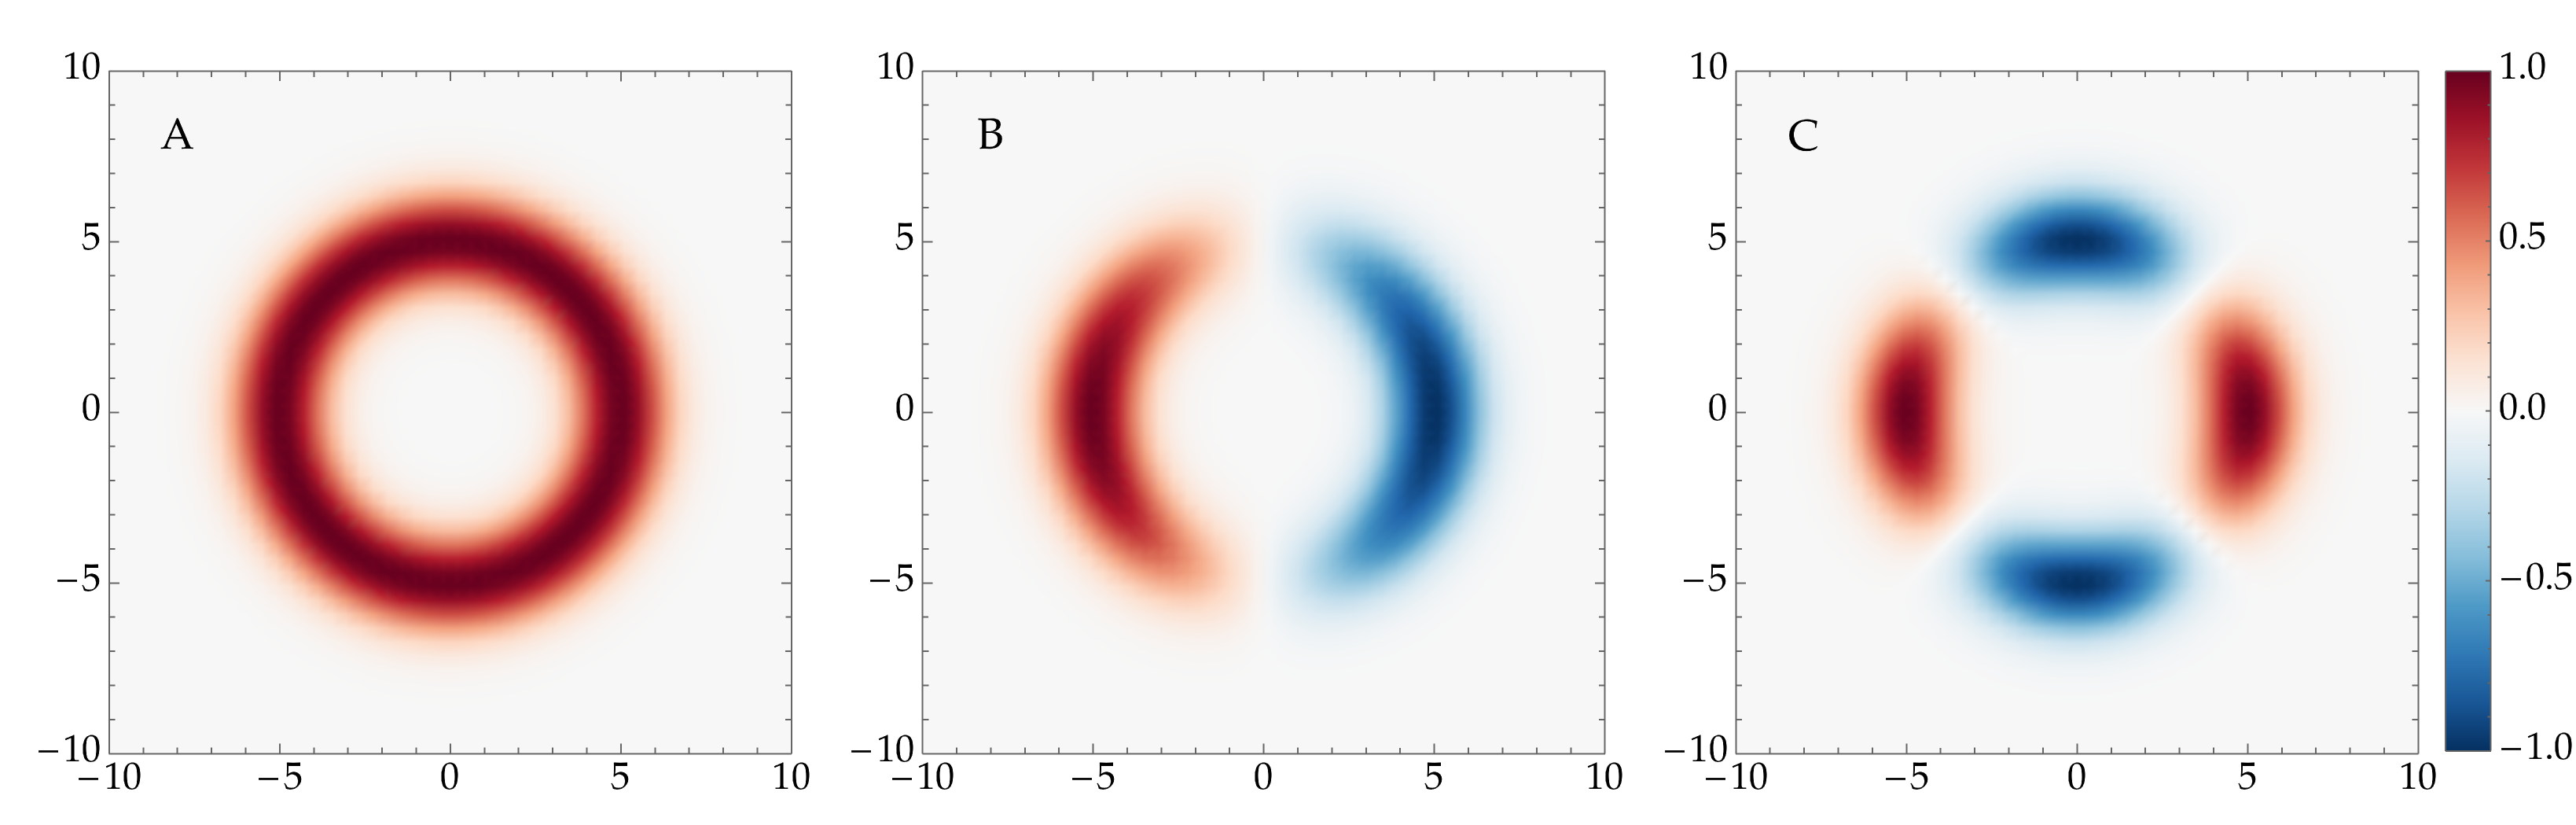
\includegraphics[width=\linewidth]{img/wave_scattering/multipolar_gaussian_id_examples.png}
  \caption{Demonstration of the multipolar Gaussian function with different parameters. For all panels, $x_0 = y_0 = z_0 = 0$ and $R_0 = 5$. In Panel \textbf{A} displays the only nonzero coefficient is $c_{00} = 1/A_{00}$, in Panel \textbf{B}, $c_{11} = 1/A_{11}$, and in Panel \textbf{C}, $c_{22} = 1/(3A_{22})$.}
  \label{fig:multipolar_gaussian_id_demo}
\end{figure}